\section{Theoretical Background}

Having established the core challenges of latency, energy efficiency, and data consistency in the previous section, this section provides the theoretical foundations necessary to understand the architectural decisions made in this thesis. It covers microservices architecture, IoT hardware constraints, communication protocols, and distributed data consistency.

\subsection{Microservices Architecture (MSA)}
Microservices Architecture (MSA) represents a fundamental shift in software design, organizing applications not as single, monolithic systems, but as suites of small, autonomous services that collaborate through well-defined interfaces \cite{awsMicroservices}. In a traditional monolithic architecture, all functionality---from user management to data processing---is tightly coupled within one large codebase. While this approach simplifies initial development, it often becomes a significant obstacle to scalability and fault tolerance as the application grows \cite{fowlerMicroservices}.

MSA addresses this limitation by treating the application as a collection of independent services, each running in its own process and communicating through lightweight channels such as HTTP APIs or messaging buses \cite{newmanBuilding}. Each service is responsible for a specific business domain. For the ``Plant Up!'' platform, this architectural style is particularly well-suited, as it allows distinct parts of the system to be built and scaled independently. For example, the service responsible for ingesting thousands of sensor readings per minute can be scaled horizontally during peak activity without affecting the social feed service, which may experience lower load at that time.

The ``Plant Up!'' backend is organized around domain-specific schemas in Supabase, which serve as the dedicated data stores for these microservices:
\begin{itemize}
    \item \texttt{user\_schema}: Manages user identity, authentication, and personal statistics such as streaks.
    \item \texttt{social\_media\_schema}: Manages the community features, including posts and comments.
    \item \texttt{gamification}: Contains the logic for quests, experience points (XP), and rewards.
    \item \texttt{microcontroller\_schema}: A high-throughput data store dedicated to raw sensor data from the IoT devices.
\end{itemize}

A clear example of this separation is the storage of sensor readings, which reside in an isolated table, entirely separate from the user data:

\begin{figure}[H]
    \centering
    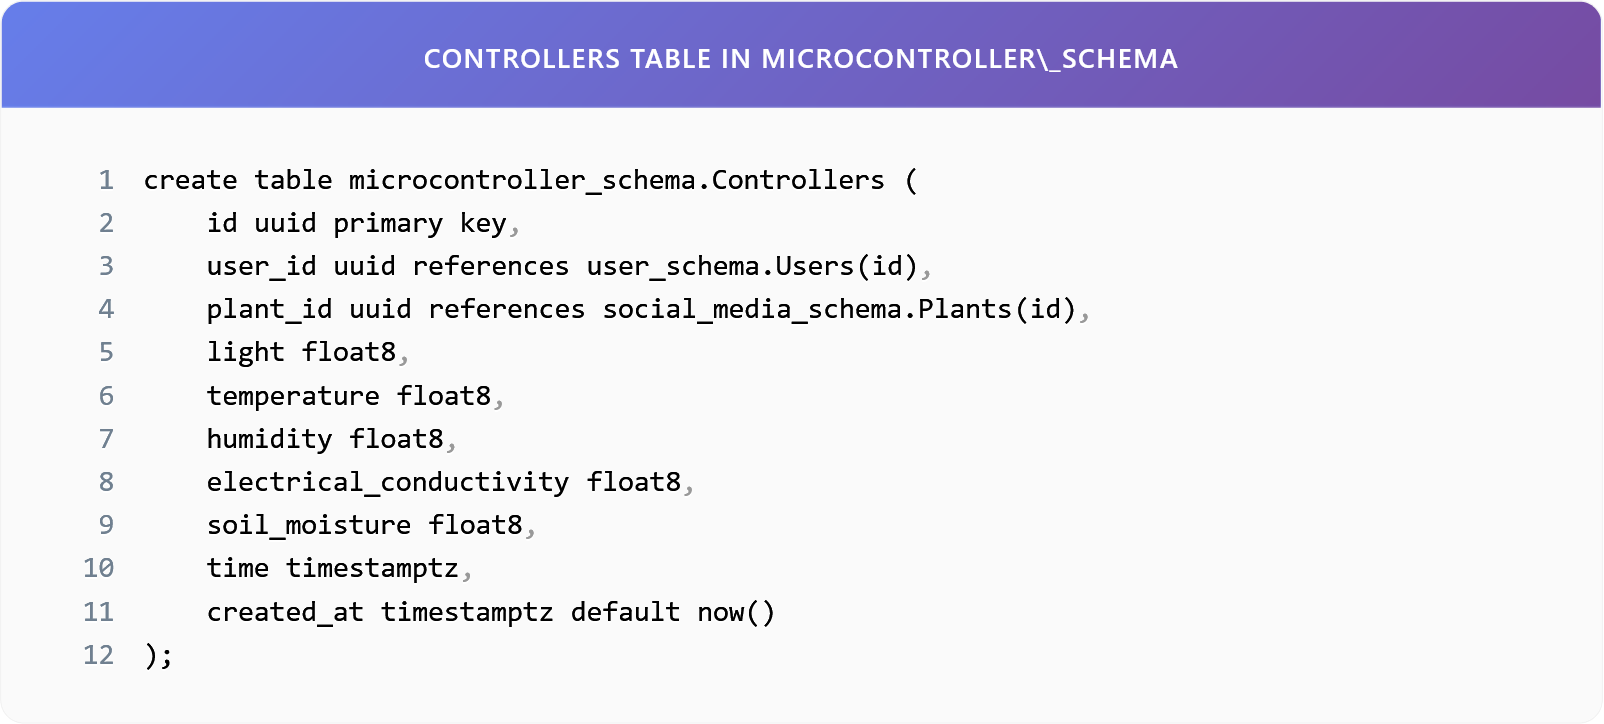
\includegraphics[width=0.8\textwidth]{images/controllers_table.png}
    \caption{Controllers table in microcontroller\_schema}
    \label{fig:controllers_table}
\end{figure}

This strict boundary improves system robustness. If the sensor reading service encounters a failure, it does not propagate to the gamification or social features.

\subsection{Core Characteristics of Microservices in IoT}
Applying Microservices Architecture to the Internet of Things brings a unique set of challenges. IoT systems are inherently asynchronous, event-driven, and must contend with the unpredictable nature of physical environments.

\subsubsection{Autonomy and Database per Service}
One of the fundamental principles of MSA is ``Database per Service''. This principle dictates that services are decoupled not only in their code, but also in their data state \cite{richardsonDbPerService}. It prevents the hazardous situation where modifying a database table for one service inadvertently breaks another. In ``Plant Up!'', the Gamification Service maintains its own independent record of player statistics, which is entirely separate from the raw stream of incoming sensor data.

\begin{figure}[H]
    \centering
    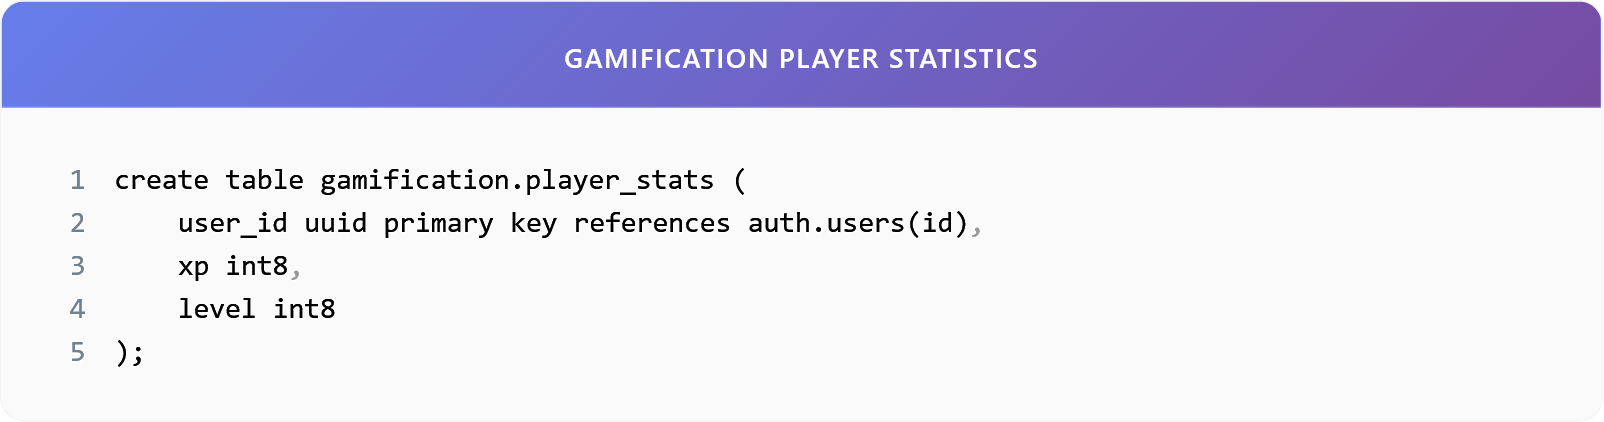
\includegraphics[width=0.8\textwidth]{images/gamification_stats.png}
    \caption{Gamification player statistics}
    \label{fig:gamification_stats}
\end{figure}

\subsubsection{Scalability and Elasticity}
IoT workloads are characteristically intermittent. Long periods of silence may be followed by sudden bursts of activity when thousands of devices wake up to report their status. MSA enables this to be handled by scaling the Ingestion Service horizontally---adding more instances to distribute the load---without allocating unnecessary resources to the Social Service, which may not require additional capacity.

\subsection{Internet of Things (IoT) Constraints and Hardware}
At the hardware level of ``Plant Up!'' is the ESP32-S3 microcontroller, a capable System-on-Chip (SoC) from Espressif Systems \cite{esp32s3Datasheet}. Despite its processing power, it remains bound by the constraints of battery life. The choice of software protocol directly determines how long the hardware remains in an active state, and consequently, how long the battery lasts.

\subsubsection{Power Consumption and Sleep Modes}
The ESP32-S3 provides several power modes, each with vastly different energy consumption characteristics. Understanding these modes is essential for the architectural design:
\begin{itemize}
    \item Active Mode: All components---CPU, Wi-Fi radio, and peripherals---are fully powered. The device consumes between 160\,mA and 260\,mA \cite{lastMinuteActive}. Minimizing time spent in this mode is critical for energy conservation.
    \item Modem Sleep: The CPU remains active, but the radio is disabled. Power consumption drops to approximately 20--30\,mA \cite{lastMinuteActive}.
    \item Deep Sleep: The CPU, Wi-Fi module, and RAM are powered down. Only the Ultra-Low Power (ULP) coprocessor and the Real-Time Clock remain active. Consumption is reduced to 10\,\textmu A--150\,\textmu A \cite{esp32s3Datasheet}.
\end{itemize}

\subsubsection{The Wake-Up Tax}
Deep sleep provides substantial energy savings, but it introduces a ``wake-up tax''. Upon waking, the device must re-initialize its Wi-Fi module, locate the access point, and negotiate an IP address. This process typically requires 1 to 3 seconds, consuming approximately 150\,mA on average before any data is transmitted \cite{adafruitWake}. The choice of communication protocol (MQTT vs.\ REST) determines how much additional overhead this process incurs.

\subsection{Communication Protocols: MQTT vs. REST}
The selection of a communication protocol is one of the most critical architectural decisions for the data layer, as it directly affects energy efficiency, latency, and reliability. This subsection examines the two protocols under consideration for the ``Plant Up!'' sensor layer.

\subsubsection{MQTT (Message Queuing Telemetry Transport)}
MQTT is a lightweight, binary messaging protocol designed specifically for networks that are unreliable or have limited bandwidth \cite{psiborg2024mqtt}. It operates on a publish-subscribe model.

Architecture and Decoupling:
Unlike REST, which connects two endpoints directly, MQTT introduces a Broker as an intermediary. The sensor (Publisher) sends data to a topic (e.g., \texttt{plantup/sensor/01}) without knowledge of which services are consuming the data. The Broker handles message routing to all subscribed services (such as the Ingestion Service). This architecture decouples the devices in space (they do not need to know each other's IP addresses) and time (messages can be queued if a service is temporarily unavailable).

\begin{figure}[H]
    \centering
    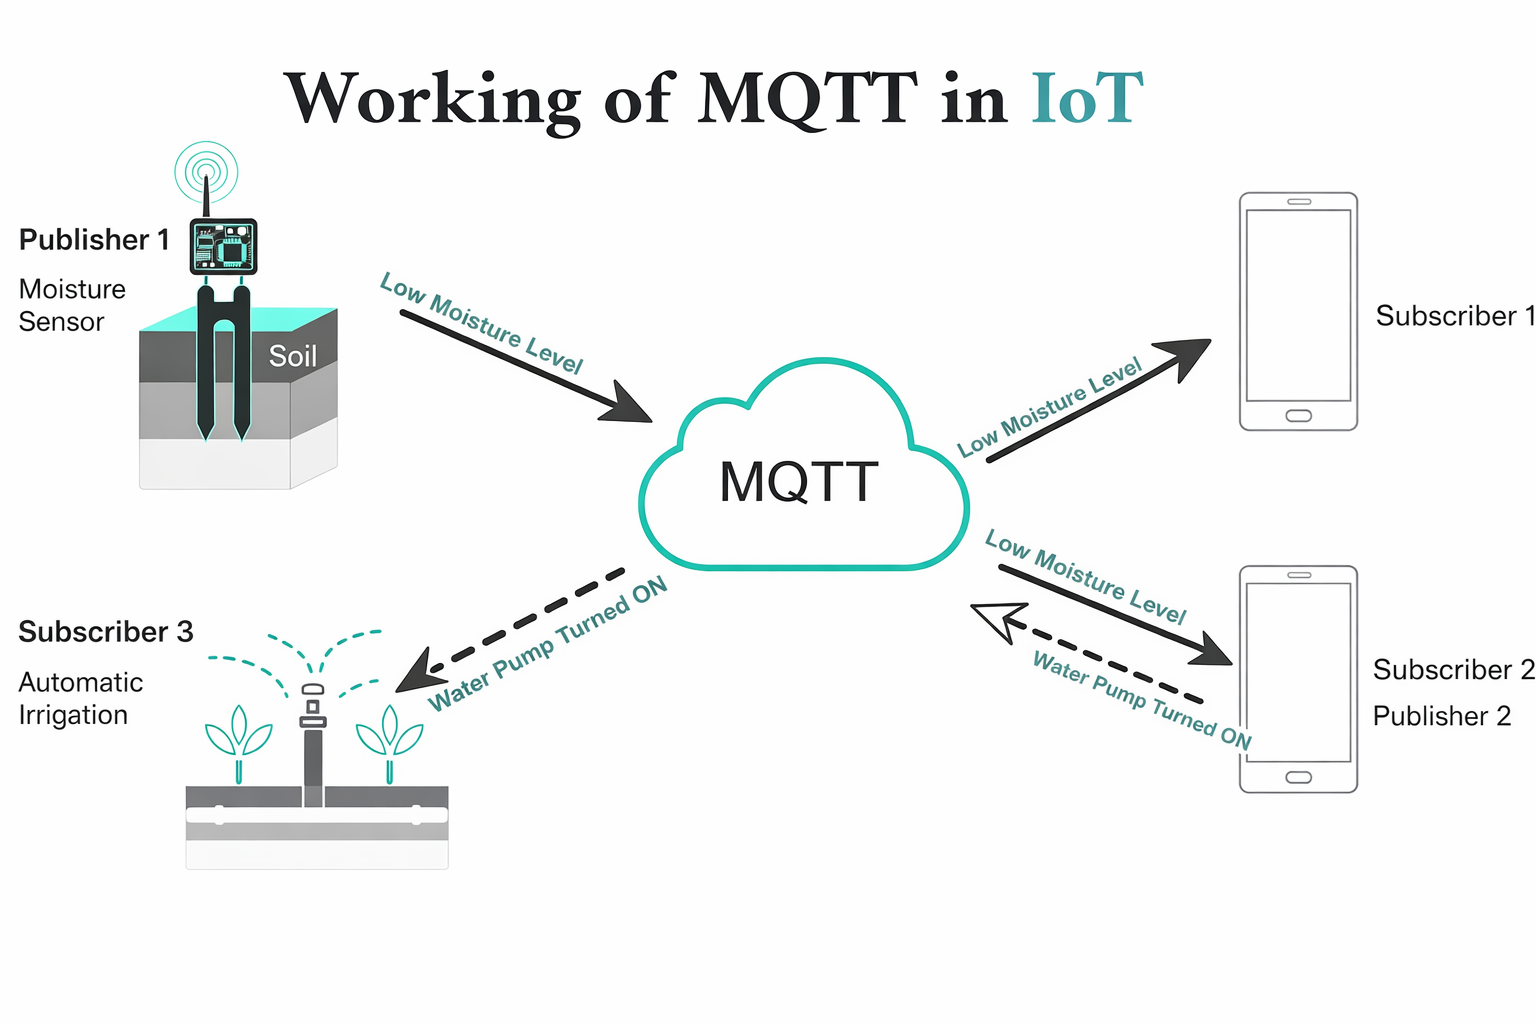
\includegraphics[width=0.8\textwidth]{images/mqtt_converted.png}
    \caption{MQTT Publish/Subscribe Model: The Broker acts as a central hub, efficiently distributing messages from sensors to various services \cite{psiborg2024mqtt}.}
    \label{fig:mqtt_diagram}
\end{figure}

Packet Structure:
MQTT uses a binary format, which eliminates textual overhead. The fixed header is only 2 bytes, in contrast to text-based HTTP headers, which can easily exceed several hundred bytes.

Quality of Service (QoS):
MQTT provides three levels of delivery assurance:
\begin{itemize}
    \item QoS 0 (At most once): A fire-and-forget approach. It consumes the least energy, but if a message is lost, it cannot be recovered.
    \item QoS 1 (At least once): Guarantees delivery by requiring an acknowledgment (PUBACK). This level is suitable for critical sensor data.
    \item QoS 2 (Exactly once): A four-step handshake that guarantees exactly-once delivery. This level typically introduces too much overhead for battery-powered devices.
\end{itemize}

\subsubsection{REST (Representational State Transfer)}
REST is the standard architectural style of the web, utilizing standard HTTP methods. It follows a synchronous, resource-oriented model.

Request-Response Model:
REST follows a strict client-server paradigm. The client issues a request (GET or POST) and waits for the server to respond before proceeding.

\begin{figure}[H]
    \centering
    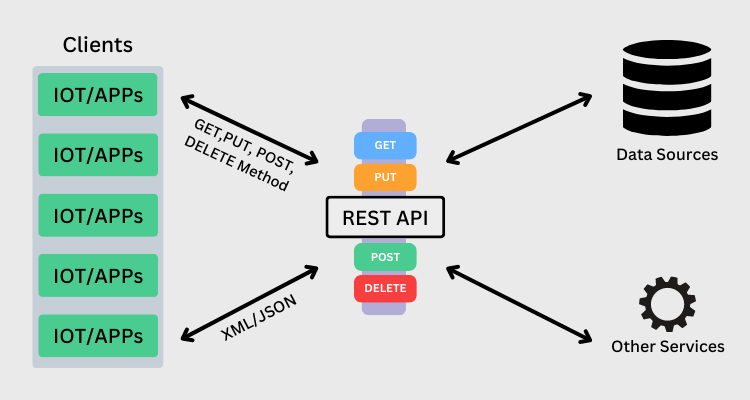
\includegraphics[width=0.8\textwidth]{images/rest_converted.png}
    \caption{REST Request-Response Workflow: Stateless clients must establish a new connection for every request, incurring significant overhead \cite{dreamfactory2024rest}.}
    \label{fig:rest_diagram}
\end{figure}

Statelessness and Overhead:
The server retains no state between requests. Consequently, every request must carry all necessary context (authentication tokens, headers, and metadata). Furthermore, if the device enters sleep between readings, it must perform a full TCP three-way handshake and frequently a TLS handshake for \textit{every single data transmission}. This connection overhead makes REST significantly less energy-efficient than a persistent MQTT session for frequent, small data packets.

\subsection{Data Consistency and the CAP Theorem}
In distributed systems, the CAP theorem (Consistency, Availability, Partition Tolerance) establishes that all three properties cannot be guaranteed simultaneously during a network failure \cite{brewerCap, jaiswalCAP}.

For ``Plant Up!'', Partition Tolerance (P) is non-negotiable, as wireless sensor networks are inherently unreliable. This necessitates a choice between CP and AP:
\begin{itemize}
    \item CP (Consistency + Partition Tolerance): Requests are rejected if data consistency cannot be guaranteed, which risks data loss during network disruptions.
    \item AP (Availability + Partition Tolerance): Data is accepted and requests are served even if some nodes are temporarily out of synchronization.
\end{itemize}

``Plant Up!'' adopts an AP design, embracing Eventual Consistency. It is acceptable for a user to observe a soil moisture value that is a few seconds old, provided the application remains responsive and stable. The MQTT broker serves as a buffer, holding messages during network disruptions and ensuring they eventually reach the microservices layer.

With the theoretical foundations now established, the following section presents the concrete system architecture of ``Plant Up!'' and demonstrates how these principles are applied in practice.
